\pdfminorversion=7
\documentclass[10pt,letterpaper]{article}
\usepackage[margin=0.9in]{geometry}
\usepackage{needspace}
\usepackage[T1]{fontenc}
\usepackage{lmodern}
\input{glyphtounicode}
\pdfgentounicode=1
\usepackage{amsmath,amssymb,bm,booktabs,graphicx,siunitx,array,longtable,setspace,xurl,hyperref,caption,placeins,etoolbox}
\usepackage[expansion=false]{microtype}
\hypersetup{
  hidelinks,
  pdftitle={Supplementary material: Correcting frozen-state curvature in inverse physics-informed neural networks via regularized state elimination},
  pdfauthor={Ziwei Ren, Shijin Zhang, Ming Chen, Chuangrui Zheng}
}
\robustify\bfseries
\sisetup{group-digits=false,detect-weight=true,detect-family=true}
\captionsetup{font=small,labelfont=bf}
\setstretch{1.06}\raggedbottom
\setlength{\emergencystretch}{2em}
\setcounter{topnumber}{3}\setcounter{totalnumber}{5}
\renewcommand{\topfraction}{.92}\renewcommand{\textfraction}{.06}
\renewcommand{\floatpagefraction}{.78}
\renewcommand{\thesection}{S\arabic{section}}
\renewcommand{\thetable}{S\arabic{table}}
\renewcommand{\thefigure}{S\arabic{figure}}
\renewcommand{\theequation}{S\arabic{equation}}
\newcommand{\Esa}{E_{\mathrm{SAEPS}}}
\newcommand{\Fraw}{F_{\mathrm{raw}}}
\newcommand{\Hred}{H_{\mathrm{red},\gamma}^{\mathrm{exact}}}
\newcommand{\Cexact}{C_{\mathrm{relax}}^{\mathrm{exact}}}
\title{Supplementary material\\[4pt]\large Correcting frozen-state curvature in inverse physics-informed neural networks via regularized state elimination}
\author{Ziwei Ren, Shijin Zhang, Ming Chen, and Chuangrui Zheng}
\date{}
\begin{document}
\maketitle
\noindent This supplement provides complete cohort records, numerical acceptance criteria, damping and undamped-limit audits, matched-damping solver timing ledgers, and operator-scale experiment details accompanying the main manuscript.
Source code, processed benchmark tables, figure- and table-generation scripts, algebraic verification tests, and experimental logs are available at \url{https://github.com/milumilelu/SAEPS}.

\section{Cohort overview and numerical conventions}
\begin{table}[!htbp]
\centering\small
\caption{Summary of experimental cohorts and analytical audits. Sample counts are kept separate across distinct targets and shared base fits.}
\begin{tabular}{p{.23\linewidth}p{.26\linewidth}p{.43\linewidth}}
\toprule
Cohort / Audit & Planned records & Role in manuscript\\\midrule
Affine scalar PDEs & 15 Burgers; 10 Allen--Cahn & Primary matched finite-damping curvature comparison\\
Exact decomposition & 12 Burgers; 9 Allen--Cahn & Exact-block error-budget and dominance-condition analysis\\
Burgers stress suite & 45 noise--sparsity; 15 architecture & Stress boundaries and 15 designated exact-Hessian anchors\\
Coupled system & 10 checkpoints (8 valid) & Availability-limited two-parameter matrix comparison\\
Five-case profile study & 5 checkpoints (1 valid) & Small-radius nonlinear-profile consistency check\\
Non-affine saturation & 8 development; 24 held-out & Non-affine coefficient extension across six held-out data seeds\\
Architecture scaling & 18 fits (6 shared with saturation) & Paired trained networks at $n_\theta\in\{65,129,337\}$\\
Saturation profile study & 21 steps; 126 branch refinements & Finite-displacement agreement vs.\ strict stationarity audit\\
Matched-damping cost & 2 centers $\times$ 4 $\alpha$ $\times$ 3 solvers $\times$ 3 repeats & Wall-clock solver cost and dense-reference agreement\\
Algebraic energy audit & Synthetic matrix tests & Exact-arithmetic verification of Proposition~2\\
\bottomrule
\end{tabular}
\end{table}

All primary scalar curvature errors are computed on the summed weighted least-squares objective $\ell=\tfrac12\|\bar{\bm r}\|_2^2$.
Because training minimizes the mean objective $\ell/m$ over $m$ residuals, curvature blocks and damping $\gamma$ scale by $m$ between the two conventions; any mean-loss implementation must divide both curvature matrices and $\gamma$ by $m$.
State refinement is performed with the fitted physical parameter $\lambda_0$ held fixed, so the resulting checkpoint satisfies approximate state stationarity rather than joint state--parameter optimality.

The primary scalar error denominator is $|\Hred|+10^{-8}$, whereas the relaxation-correction error $E_{\rm relax}$ uses $|\Cexact|+10^{-8}$; these two normalizations answer different questions and are reported separately.
The finite-step profile discrepancy uses $\max(|\Hred|,10^{-8})$, and the coupled two-parameter matrix metric is defined in Section~\ref{sec:coupled}.

\begin{table}[!htbp]
\centering\small
\caption{Prespecified numerical acceptance rules for the affine scalar benchmarks.}
\begin{tabular}{p{.36\linewidth}p{.56\linewidth}}
\toprule
Check & Criterion\\\midrule
Local state-gradient refinement & Normalized mean-objective gradient $g_\theta^{\rm norm}\le 10^{-6}$\\
Final center stationarity & $g_\theta^{\rm norm}<10^{-4}$ and $s_\theta<10^{-4}$\\
Nominal damping & $\gamma=10^{-8}\lambda_{\max}(J_\theta^\top J_\theta)$\\
Iterative state solve & Scaled augmented LSQR; tolerance $10^{-10}$; iterative refinement\\
Linear-solve acceptance & Verified normal residual $\le10^{-8}$; explicit-curvature discrepancy $\le10^{-6}$\\
Exact-Hessian symmetry & Relative tolerance $10^{-8}$\\
Damped state reference & Positive-eigenvalue relative tolerance $10^{-10}$; solve residual $\le10^{-8}$\\
Burgers cohort target & 15 planned; at least 12 valid and 12 planned improvements\\
Allen--Cahn cohort target & 10 planned; at least 8 valid and 8 planned improvements\\
Sign-test rule & Positive paired median and one-sided exact sign test at $0.05$\\
Invalid checkpoint handling & Retained in planned denominator; omitted from conditional error summaries\\
\bottomrule
\end{tabular}
\end{table}

A small gradient norm is a local stationarity indicator rather than a certified distance to a local minimum, and the local Newton step $-(H_{\theta\theta}+\gamma I)^{-1}g_\theta$ does not provide a global state-error bound.
For the Burgers and Allen--Cahn cohorts, all processed curvature blocks and summary records are preserved for independent reproduction, whereas original unarchived state tensors from those earlier training runs are not retained for tensor-level replay; reconstructed tensors are never substituted for the original checkpoints.

\Needspace{7\baselineskip}
\section{Complete affine scalar records}
\begin{longtable}{lScSS}
\caption{Complete affine scalar cohorts (Burgers and Allen--Cahn). Invalid centers remain in the planned denominator.}\label{tab:historical_all}\\
\toprule
Problem & {Seed} & Status & {$E_{\rm raw}$} & {$E_{\rm SAEPS}$} \\
\midrule\endfirsthead
\toprule
Problem & {Seed} & Status & {$E_{\rm raw}$} & {$E_{\rm SAEPS}$} \\
\midrule\endhead
Burgers & 55 & valid & 22.2045 & 0.0789617 \\
Burgers & 56 & valid & 19.9879 & 0.0922864 \\
Burgers & 57 & invalid & {--} & {--} \\
Burgers & 58 & valid & 28.7944 & 0.0142054 \\
Burgers & 59 & valid & 25.5988 & 0.021715 \\
Burgers & 60 & valid & 27.4137 & 0.0967368 \\
Burgers & 61 & invalid & {--} & {--} \\
Burgers & 62 & valid & 30.4464 & 0.0711029 \\
Burgers & 63 & invalid & {--} & {--} \\
Burgers & 64 & valid & 23.6552 & 0.0699458 \\
Burgers & 65 & valid & 30.2836 & 0.100541 \\
Burgers & 66 & valid & 28.04 & 0.0843159 \\
Burgers & 67 & valid & 38.6729 & 0.0420263 \\
Burgers & 68 & valid & 29.8111 & 0.207051 \\
Burgers & 69 & valid & 25.2792 & 0.0551079 \\
Allen--Cahn & 75 & valid & 19.7223 & 0.244784 \\
Allen--Cahn & 76 & valid & 16.2127 & 0.119892 \\
Allen--Cahn & 77 & valid & 22.2218 & 0.390497 \\
Allen--Cahn & 78 & valid & 21.9146 & 0.281678 \\
Allen--Cahn & 79 & valid & 25.1832 & 0.466723 \\
Allen--Cahn & 80 & valid & 20.3728 & 0.366263 \\
Allen--Cahn & 81 & invalid & {--} & {--} \\
Allen--Cahn & 82 & valid & 19.3133 & 0.155524 \\
Allen--Cahn & 83 & valid & 17.7076 & 0.218192 \\
Allen--Cahn & 84 & valid & 21.9076 & 0.278567 \\
\bottomrule
\end{longtable}

The valid-checkpoint exact sign tests are conditional on passing the numerical acceptance rules in Table~S2, while planned cohort sizes remain $15$ and $10$.
Ratios of medians and medians of paired error ratios measure distinct summaries: for Burgers they equal $369.53$ and $335.38$, and for Allen--Cahn they equal $73.13$ and $78.64$.

\section{Coupled two-parameter benchmark and matrix comparison}
\label{sec:coupled}
The manufactured fields are
\begin{align}
 u^\star(x,t)&=\sin(\pi x)e^{-t}+0.1\sin(2\pi x)\sin t,\\
 v^\star(x,t)&=\cos(\pi x/2)e^{-t/2}+0.1\sin(3\pi x)\cos t,
\end{align}
substituted into the coupled reaction--diffusion system
\begin{align}
 u_t&=0.03u_{xx}-a u+b v+f_u,\\
 v_t&=0.02v_{xx}+a u-b v+f_v.
\end{align}
Sources $f_u,f_v$ are computed once at the true values $(a,b)=(0.8,0.75)$ and held fixed during inference, starting from initial estimates $(0.6,0.95)$ in logarithmic coordinates $(\log a,\log b)$.
Dirichlet boundary conditions are enforced at both spatial endpoints.
Each field is represented by an independent width-$6$ $\tanh$ network ($n_\theta=50$ state parameters jointly), with $96$ PDE points, $128$ observations, $48$ initial points, and $96$ boundary points per channel ($m=736$ residuals total).

To compare $2\times 2$ curvature matrices on a common scale, define the stabilized whitening matrix
\begin{equation}
 B=\tfrac12(F_{\rm raw}+F_{\rm raw}^{\top})+\tau I,
 \qquad \tau=10^{-10}\max\{\operatorname{tr}(F_{\rm raw})/2,1\}.
\end{equation}
With Cholesky factor $B=LL^\top$ and $\mathcal W(X)=L^{-1}XL^{-\top}$, matrix errors are defined by
\begin{equation}
 E_X^{(2)}=\frac{\|\mathcal W(F_X-H_{\rm red})\|_F}
 {\|\mathcal W(H_{\rm red})\|_F+10^{-30}}.
\end{equation}
All methods share the same metric at each checkpoint (this metric does not guarantee invariance under arbitrary nonlinear reparameterizations).

\begin{table}[!htbp]
\centering\small
\caption{All ten coupled two-parameter checkpoints. Both invalid centers fail the state-center validity gate.}
\begin{tabular}{rcrr}
\toprule
Seed & Valid & $E_{\rm raw}^{(2)}$ & $E_{\rm SAEPS}^{(2)}$\\\midrule
215 & yes & 17.3643 & 0.02593\\
216 & yes & 9.5722 & 0.02116\\
217 & yes & 14.4154 & 0.01100\\
218 & yes & 14.5991 & 0.02019\\
219 & no & -- & --\\
220 & yes & 9.2373 & 0.03854\\
221 & no & -- & --\\
222 & yes & 14.9614 & 0.02982\\
223 & yes & 15.5080 & 0.11856\\
224 & yes & 12.3405 & 0.09526\\\bottomrule
\end{tabular}
\end{table}
All eight valid checkpoints favor SAEPS (conditional exact one-sided sign test $p=3.91\times10^{-3}$, unadjusted), while the prespecified $9/10$ availability gate is not met.
Varying the whitening stabilizer $\tau$ across $[10^{-12},10^{-8}]$ preserves the paired advantage on every valid checkpoint.
Separately, algebraic coordinate-transformation identities were verified on all ten coupled checkpoints (including the two invalid centers, as algebraic identities do not require stationarity); applying the matching transformed state metric preserves linear-coordinate representations, whereas replacing it with the Euclidean identity changes the target.

\begin{table}[!htbp]
\centering
\caption{Terminal failure categories for the historical accuracy cohorts.}
\label{tab:failure_counts}
\small
\setlength{\tabcolsep}{4pt}
\begin{tabular}{l *{6}{S[table-format=2.0]}}
\toprule
{Cohort} & {Planned} & {Accepted} & {\shortstack{State\\center}} & {Solve} & {Non-finite} & {Other} \\
\midrule
Burgers & 15 & 12 & 3 & 0 & 0 & 0 \\
Allen--Cahn & 10 & 9 & 1 & 0 & 0 & 0 \\
Coupled & 10 & 8 & 2 & 0 & 0 & 0 \\
\bottomrule
\end{tabular}
\par\vspace{3pt}\begin{minipage}{.98\linewidth}\footnotesize Burgers failures are seeds 57, 61, and 63; Allen--Cahn fails at seed 81; coupled failures are 219 and 221. All are recorded as state-center acceptance failures. Counts classify the primary accuracy endpoint, not the separate profile experiments or nonbinding score diagnostics. The source aggregates are listed in the revision provenance. This classification does not assume ignorable missingness or alter historical acceptance gates.\end{minipage}
\end{table}


\section{Non-affine saturation setup, aggregation, and held-out fits}
The manufactured saturation solution is
\begin{equation}
 u^\star(x,t)=1+0.2e^{-t}\cos(2\pi x)+0.1e^{-2t}\sin(4\pi x),
\end{equation}
which satisfies $u^\star\ge 0.7$ on the domain, with fixed manufactured source
\begin{equation}
 f=u_t^\star-0.01u_{xx}^\star-\frac{u^\star}{1+1.2u^\star}.
\end{equation}
The network output uses $u=\operatorname{softplus}(v)+0.05$ with all spatial and temporal derivatives propagated through the transformation.
Zero-mean Gaussian noise is added only to observations, scaled by the standard deviation of sampled truth values, while the source $f$ remains correctly specified.

Development uses data seeds $916001$--$916002$ and held-out evaluation uses data seeds $916101$--$916106$, each paired with initialization seeds $926001$--$926002$ and observation noise levels $0$ and $0.02$ sharing spatial--temporal layouts and standard-normal draws.
Joint training runs $3000$ Adam steps ($10^{-3}$) and up to $1000$ L-BFGS iterations on the mean objective, followed by fixed-$\lambda$ state refinement capped at $100{,}000$ iterations.
During development at ceilings of $10{,}000$, $30{,}000$, and $100{,}000$ iterations, valid center counts were $6/8$, $8/8$, and $8/8$; increasing the ceiling from $30{,}000$ to $100{,}000$ altered individual relative errors by up to $14.2\%$ and shifted the development median by approximately $2.2\%$, after which the $100{,}000$-iteration budget was frozen prior to held-out execution.

\subsection{Aggregation at the independent data-seed level}
Each held-out data seed contains four dependent fits ($2$ initializations $\times$ $2$ noise levels).
The main summary pools these four fits by their seed median before taking the median across six independent data seeds (a post-hoc cross-noise pooling rule); noise-stratified summaries preserve the original within-noise initialization median.
All $24$ individual fits and all $6$ seed summaries favor SAEPS ($p=1.5625\times10^{-2}$, exact one-sided sign test, no ties, unadjusted).
Empirical quartiles in Table~S6 use linear interpolation and describe sample dispersion rather than calibrated confidence intervals.
\begin{table}[!htbp]
\centering
\caption{Paired effect sizes and empirical quartiles at the declared statistical unit.}
\label{tab:effect_sizes}
\small
\setlength{\tabcolsep}{4pt}
\begin{tabular}{l S[table-format=2.0] *{3}{S[table-format=2.3]} *{3}{S[table-format=5.1]}}
\toprule
{Cohort} & {$n$} & {$D_{25}$} & {$D_{50}$} & {$D_{75}$} & {$R_{25}$} & {$R_{50}$} & {$R_{75}$} \\
\midrule
Burgers & 12 & 24.814 & 27.636 & 29.749 & 282.8 & 335.4 & 574.1 \\
Allen--Cahn & 9 & 19.158 & 20.006 & 21.633 & 56.9 & 78.6 & 81.2 \\
Saturation & 6 & 16.532 & 16.815 & 17.753 & 10427.2 & 16883.1 & 18262.9 \\
\bottomrule
\end{tabular}
\par\vspace{3pt}\begin{minipage}{.98\linewidth}\footnotesize $D=E_{\rm raw}-E_{\rm SAEPS}$ and $R=E_{\rm raw}/E_{\rm SAEPS}$ use the same unit-level pair. Subscripts denote empirical percentiles, using linear interpolation. Historical units are accepted checkpoints; saturation units are six four-fit medians. The saturation difference is formed after that pooling. These quartiles summarize dispersion, not a bootstrap or calibrated 95\% confidence interval. No cohorts are pooled for inference.\end{minipage}
\end{table}

\begin{table}[!htbp]
\centering\small
\caption{Aggregation levels are kept consistent for both error ratios.}
\label{tab:aggregate}
\begin{tabular}{lSSSS}
\toprule
Units & {Median $E_{\rm raw}$} & {Median $E_{\rm SAEPS}$} & {$R_1$} & {$R_2$} \\
\midrule
24 individual fits & 16.8 & 0.0012466 & 13476.6 & 13257.2 \\
6 pooled seed medians & 16.817 & 0.0010603 & 15860.2 & 16883.1 \\
\bottomrule
\end{tabular}
\par\vspace{3pt}\begin{minipage}{.96\linewidth}\footnotesize $R_1$ is the ratio of medians at the stated level. $R_2$ is the median of paired error ratios at that same level. The value $13257.2$ describes individual-fit ratios, not ratios of six seed medians. The six-unit pooling is post hoc.\end{minipage}
\end{table}

\begin{table}[!htbp]
\centering
\caption{Saturation results by data seed under the reported four-fit pooling rule.}
\label{tab:e3_seeds}
\small
\setlength{\tabcolsep}{5pt}
\begin{tabular}{SSSS}
\toprule
{Data seed} & {$E_{\rm raw}$} & {$E_{\rm SAEPS}$} & {$E_{\rm GN,fix}$} \\
\midrule
916101 & 18.0619 & 0.0020743 & 0.0016737 \\
916102 & 16.8005 & 0.00092244 & 0.00083258 \\
916103 & 15.6652 & 0.00056618 & 0.00054936 \\
916104 & 18.635 & 0.0011982 & 0.0014005 \\
916105 & 16.444 & 0.00089958 & 0.00070999 \\
916106 & 16.8326 & 0.0019307 & 0.0014523 \\
\bottomrule
\end{tabular}
\par\vspace{3pt}\begin{minipage}{.98\linewidth}\footnotesize The median over four fits is an explicitly post-hoc cross-noise summary. It is not the same as taking a median after a within-noise averaging step.\end{minipage}
\end{table}

\begin{figure}[!htbp]
\centering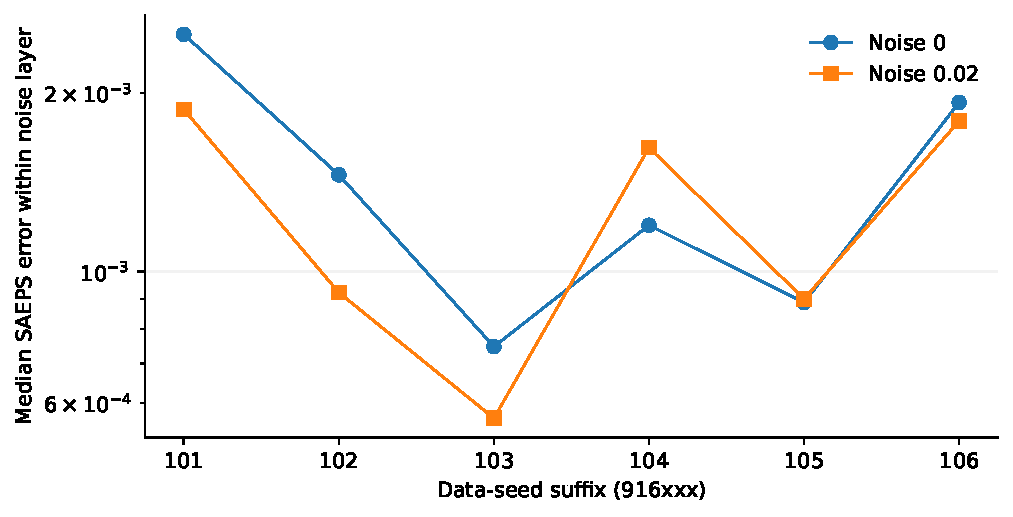
\includegraphics[width=.94\linewidth]{figures/s04_noise_stratified.pdf}
\caption{Noise-stratified saturation errors. Each point is the median of two initializations at one data seed and noise level; the two noise layers share data seeds and are not independent cohorts.}
\end{figure}
\begin{longtable}{SScSSS}
\caption{All saturation held-out fits. Init. A/B denote 926001/926002.}\label{tab:e3_all}\\
\toprule
{Data seed} & {Noise} & Init. & {$E_{\rm raw}$} & {$E_{\rm SAEPS}$} & {$E_{\rm GN,fix}$} \\
\midrule\endfirsthead
\toprule
{Data seed} & {Noise} & Init. & {$E_{\rm raw}$} & {$E_{\rm SAEPS}$} & {$E_{\rm GN,fix}$} \\
\midrule\endhead
916101 & 0 & A & 18.312 & 0.0017404 & 0.0016107 \\
916101 & 0 & B & 17.953 & 0.0032895 & 0.0028426 \\
916101 & 0.02 & A & 17.86 & 0.0013495 & 0.0012243 \\
916101 & 0.02 & B & 18.171 & 0.0024082 & 0.0017366 \\
916102 & 0 & A & 16.778 & 8.7904e-06 & 0.00012477 \\
916102 & 0 & B & 16.823 & 0.0029059 & 0.0020027 \\
916102 & 0.02 & A & 16.579 & 0.00089511 & 0.00093129 \\
916102 & 0.02 & B & 17.014 & 0.00094978 & 0.00073388 \\
916103 & 0 & A & 15.692 & 0.00026875 & 7.2709e-05 \\
916103 & 0 & B & 15.71 & 0.0012266 & 0.0009995 \\
916103 & 0.02 & A & 15.639 & 0.00077609 & 0.00068765 \\
916103 & 0.02 & B & 15.602 & 0.00035627 & 0.00041107 \\
916104 & 0 & A & 18.483 & 0.0012455 & 0.0012291 \\
916104 & 0 & B & 18.635 & 0.0011508 & 0.0015719 \\
916104 & 0.02 & A & 18.701 & 0.00065472 & 0.00018758 \\
916104 & 0.02 & B & 18.635 & 0.0025846 & 0.0026048 \\
916105 & 0 & A & 16.492 & 0.0015443 & 0.0013698 \\
916105 & 0 & B & 16.363 & 0.00023097 & 0.00042181 \\
916105 & 0.02 & A & 16.443 & 0.00055134 & 0.00032313 \\
916105 & 0.02 & B & 16.445 & 0.0012478 & 0.00099817 \\
916106 & 0 & A & 16.941 & 0.0020306 & 0.0012626 \\
916106 & 0 & B & 16.705 & 0.0018307 & 0.0017752 \\
916106 & 0.02 & A & 16.724 & 0.0012594 & 0.0011371 \\
916106 & 0.02 & B & 16.963 & 0.0023341 & 0.001642 \\
\bottomrule
\end{longtable}


\section{Trained architecture scaling and dominance-condition audit}
All three trained architectures ($n_\theta\in\{65,129,337\}$) use noise level $0.02$, data seeds $916101$--$916103$, and both initialization seeds.
The six base ($n_\theta=65$) fits are shared with the main saturation cohort, and the wider ($129$) and deeper ($337$) networks contribute twelve additional trained fits.
Every valid accuracy record across the study passes its cohort's damped state-block positivity and linear-solve checks ($12/15$ Burgers, $9/10$ Allen--Cahn, $8/10$ coupled, $24/24$ saturation, and $18/18$ architecture records).
At $n_\theta=337$, the largest dense-Hessian versus HVP discrepancy across tested directions is $1.54\times10^{-15}$.

\begin{table}[!htbp]
\centering
\caption{Paired curvature errors across trained architectures on the saturation problem. Bold entries denote the lower median error per architecture.}
\label{tab:architecture}
\small
\setlength{\tabcolsep}{4pt}
\begin{tabular}{l S[table-format=3.0] c S[table-format=2.4] S[table-format=1.3e-1,scientific-notation=true] S[table-format=1.6]}
\toprule
{Architecture} & {$n_\theta$} & {Valid} & {Median $E_{\rm raw}$} & {Median $E_{\rm SAEPS}$} & {Coefficient error} \\
\midrule
2--16--1 & 65 & 6/6 & 16.797 & \bfseries 0.0009224 & 0.01302 \\
2--32--1 & 129 & 6/6 & 16.931 & \bfseries 0.0006087 & 0.007905 \\
2--16--16--1 & 337 & 6/6 & 17.266 & \bfseries 0.0004322 & 0.004592 \\
\bottomrule
\end{tabular}
\par\vspace{3pt}\begin{minipage}{.98\linewidth}\footnotesize Each architecture evaluates three data seeds and two initializations at observation noise $0.02$. The six base ($n_\theta=65$) fits are shared with the main saturation cohort; twelve wider and deeper fits are additional. The rightmost column reports the median parameter error $|\widehat\kappa-\kappa^\star|/\kappa^\star$ of the underlying PINN fits, which post-training SAEPS leaves unchanged.\end{minipage}
\end{table}

\begin{table}[!htbp]
\centering\small
\caption{Realized state-refinement iterations and training wall-clock times across architectures.}
\label{tab:arch_resources}
\begin{tabular}{SSSSSS}
\toprule
{$n_\theta$} & {Min. iterations} & {Max. iterations} & {Median iterations} & {Median fit time (s)} & {Max. $g_\theta^{\rm norm}$} \\
\midrule
65 & 65067 & 71962 & 70348 & 272.184 & 8.67e-08 \\
129 & 67488 & 88948 & 75999.5 & 526.201 & 6.633e-08 \\
337 & 65183 & 100000 & 69430.5 & 370.882 & 7.828e-08 \\
\bottomrule
\end{tabular}
\end{table}

The reported parameter errors characterize the underlying PINN fits, which post-training SAEPS leaves unchanged.
Although two width-$32$ fits have slightly larger SAEPS errors than their paired width-$16$ counterparts, all $18/18$ fits improve over their frozen-state baselines by roughly four orders of magnitude.

Evaluating Corollary~1 of the main manuscript,
\begin{equation}
 \chi=\frac{2|F_{\rm raw}-H_{\rm fix}|+
 |(F_{\rm raw}-F_{\rm se})-(H_{\rm fix}-H_{\rm red})|}
 {|H_{\rm fix}-H_{\rm red}|},
\end{equation}
confirms that all $39/39$ valid scalar checkpoints satisfy $\chi<1$:
Burgers ($12/12$: $\chi\in[0.00811,0.02596]$, median $0.01526$),
Allen--Cahn ($9/9$: $\chi\in[0.02285,0.04565]$, median $0.03293$),
and the $18$ saturation architecture checkpoints ($\max\chi=4.706\times10^{-4}$).
Because computing $\chi$ requires exact reference blocks, Corollary~1 serves as an explanatory mechanism check rather than a reference-free deployment predictor.

\section{Finite-step profile agreement and stationarity boundaries}
For the saturation profile study, the anchor $\theta_0$ and numerical damping $\gamma$ are held fixed while $\lambda$ is displaced symmetrically in log coordinates across three data seeds and seven step sizes ($21$ symmetric differences $D_\gamma(h;1)$).
Three graded state-gradient tolerances ($10^{-8}$, $10^{-10}$, and $10^{-12}$) are applied to both $\pm h$ branches ($126$ refinement runs total, with a $1000$-iteration per-point cap and a $2\text{-hour}$ per-center wall cap).
Writing $d_\pm=\|\widehat\theta_\pm-\theta_0\|_2$, all $21$ pairs pass the displacement-comparability screen $|d_+-d_-|<10\max(d_+,10^{-30})$ (a norm-asymmetry check that does not certify a shared nonlinear basin), and $20/21$ agree with $\Hred$ within $10\%$ under $|D_\gamma(h;1)-\Hred|/\max(|\Hred|,10^{-8})$.
However, $0/21$ branch pairs reach the strictest gradient tolerance and only $5/126$ individual refinements meet their assigned graded threshold.
\begin{longtable}{SSSSS}
\caption{All $21$ saturation finite-step profile differences with local Schur references and relative discrepancies.}\label{tab:profile_all}\\
\toprule
{Data seed} & {$h$} & {$D_\gamma(h;1)$} & {$H_{\rm red}$} & {Relative difference} \\
\midrule\endfirsthead
\toprule
{Data seed} & {$h$} & {$D_\gamma(h;1)$} & {$H_{\rm red}$} & {Relative difference} \\
\midrule\endhead
916101 & 0.1 & 1.67669 & 1.679225 & 0.0015095 \\
916101 & 0.03 & 1.678992 & 1.679225 & 0.00013891 \\
916101 & 0.01 & 1.679193 & 1.679225 & 1.9085e-05 \\
916101 & 0.003 & 1.678778 & 1.679225 & 0.00026625 \\
916101 & 0.001 & 1.679162 & 1.679225 & 3.7887e-05 \\
916101 & 0.0003 & 1.677717 & 1.679225 & 0.00089836 \\
916101 & 0.0001 & 1.672139 & 1.679225 & 0.0042199 \\
916102 & 0.1 & 1.688008 & 1.690765 & 0.001631 \\
916102 & 0.03 & 1.687768 & 1.690765 & 0.0017729 \\
916102 & 0.01 & 1.651275 & 1.690765 & 0.023356 \\
916102 & 0.003 & 1.689393 & 1.690765 & 0.00081168 \\
916102 & 0.001 & 1.688508 & 1.690765 & 0.0013353 \\
916102 & 0.0003 & 1.667385 & 1.690765 & 0.013829 \\
916102 & 0.0001 & 1.494485 & 1.690765 & 0.11609 \\
916103 & 0.1 & 1.768964 & 1.771738 & 0.0015659 \\
916103 & 0.03 & 1.771443 & 1.771738 & 0.0001667 \\
916103 & 0.01 & 1.771637 & 1.771738 & 5.7233e-05 \\
916103 & 0.003 & 1.771645 & 1.771738 & 5.2398e-05 \\
916103 & 0.001 & 1.771459 & 1.771738 & 0.00015757 \\
916103 & 0.0003 & 1.76955 & 1.771738 & 0.0012348 \\
916103 & 0.0001 & 1.755291 & 1.771738 & 0.009283 \\
\bottomrule
\end{longtable}


\begin{table}[!htbp]
\centering\small
\caption{Separate five-case nonlinear-profile consistency benchmark.}
\begin{tabular}{rcrr}
\toprule
Seed & Profile valid & Finest relative error & Last-two change\\\midrule
200 & no & 0.794058 & 0.0984479\\
201 & no & 1.73825 & 1.08349\\
202 & no & 0.272789 & 0.554042\\
203 & no & 0.101858 & 0.159299\\
204 & yes & 0.0538669 & 0.0010568\\\bottomrule
\end{tabular}
\end{table}
In this separate five-case benchmark, only $1/5$ checkpoints passed both small-radius consistency gates, reinforcing the main manuscript's distinction between local exact-Hessian Schur agreement and globally converged multiscale profile equivalence.

\section{Finite-damping sweep and stress boundaries}
\begin{table}[!htbp]
\centering\small
\caption{Finite-damping sweep across six fixed Burgers and Allen--Cahn centers. Only two centers resolve at $\alpha=10^{-10}$, so that row summarizes a different resolved subset.}
\label{tab:damping_sweep}
\begin{tabular}{rcrrr}
\toprule
$\alpha$ & Resolved & Median retained fraction & Median effective rank & Median $E_{\rm SAEPS}$\\\midrule
$10^{-10}$ & 2/6 & 0.0456 & 41.1599 & 0.2588\\
$10^{-8}$ & 6/6 & 0.0483 & 35.7827 & 0.1630\\
$10^{-6}$ & 6/6 & 0.0653 & 27.0456 & 0.1379\\
$10^{-4}$ & 6/6 & 0.1301 & 16.3312 & 0.0602\\
$10^{-2}$ & 6/6 & 0.5798 & 6.5750 & 0.0185\\
$1$ & 6/6 & 0.9688 & 0.9495 & 0.0116\\
$100$ & 6/6 & 0.9996 & 0.0152 & 0.0112\\\bottomrule
\end{tabular}
\end{table}
The nominal damping scale remains fixed at $\alpha=10^{-8}$ throughout the primary accuracy experiments.
Because increasing $\alpha$ changes $\gamma$ and continuously shifts the target $\Hred$ toward $\Fraw$, values of $E_{\rm SAEPS}$ across different rows of Table~\ref{tab:damping_sweep} are not directly comparable and were not used to tune $\alpha$.

\begin{figure}[!htbp]
\centering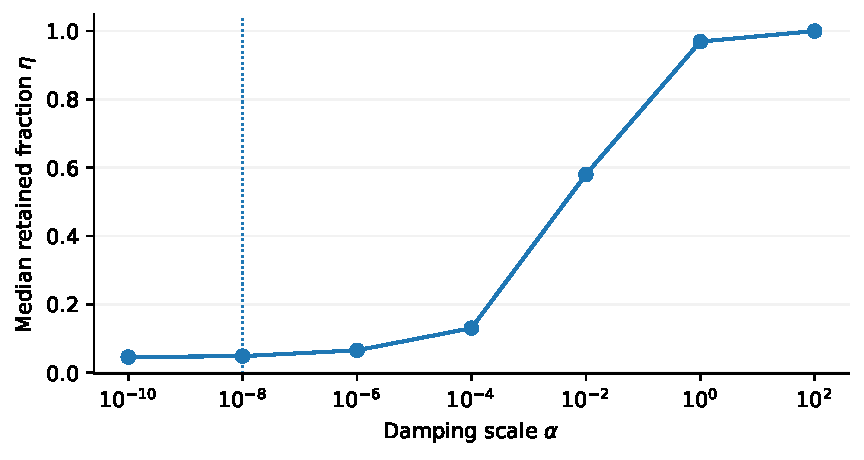
\includegraphics[width=.92\linewidth]{figures/s01_retained_fraction.pdf}
\caption{Median retained curvature fraction $\eta$ approaches the frozen-state limit as damping increases ($2/6$ resolved at $\alpha=10^{-10}$; $6/6$ at all larger $\alpha$).}
\end{figure}
\begin{figure}[!htbp]
\centering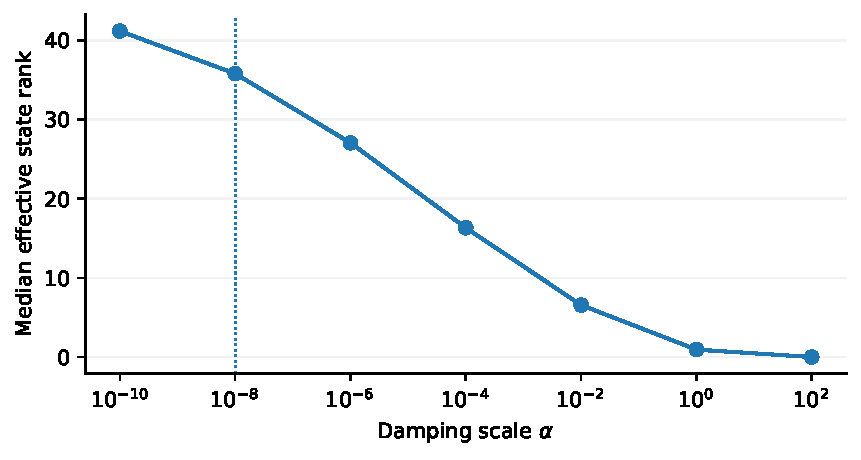
\includegraphics[width=.92\linewidth]{figures/s02_effective_rank.pdf}
\caption{Median effective state rank $r_{\rm eff}(\gamma)$ decreases monotonically with stronger damping across the same six-center sweep.}
\end{figure}

The Burgers stress campaign crosses observation noise levels $\{0, 0.01, 0.05\}$ with observation fractions $\{1.0, 0.5, 0.2\}$ ($128$, $64$, and $26$ sensors) across five seeds ($130$--$134$), yielding $43/45$ valid records.
Exact-Hessian anchors are evaluated at three cells---$(0,1.0)$, $(0.01,0.5)$, and $(0.05,0.2)$---with $14/15$ valid checkpoints, all favoring SAEPS (median error $38.1318\to 0.0879$).
A separate Burgers width sweep across widths $8$, $16$, and $32$ (seeds $135$--$139$) yields $5/5$, $4/5$, and $0/5$ valid centers, respectively ($52/60$ valid overall across both stress campaigns, with $7$ center failures and $1$ solver failure retained).

\begin{table}[!htbp]
\centering\small
\caption{All fourteen accepted historical exact-Hessian stress anchors, retained at the original displayed precision.}
\label{tab:stress_anchors}
\begin{tabular}{SSSS}
\toprule
{Anchor} & {$H_{\rm red}$} & {$E_{\rm raw}$} & {$E_{\rm SAEPS}$} \\
\midrule
1 & 38.1954 & 21.6755 & 0.0788 \\
2 & 13.8935 & 93.6491 & 0.1165 \\
3 & 25.6840 & 34.6225 & 0.1349 \\
4 & 22.5017 & 51.0975 & 0.0511 \\
5 & 16.3872 & 77.6916 & 0.0123 \\
6 & 44.2325 & 18.9195 & 0.0825 \\
7 & 34.7211 & 28.3335 & 0.0535 \\
8 & 17.8881 & 50.7631 & 0.4012 \\
9 & 39.8686 & 25.9028 & 0.1183 \\
10 & 35.4153 & 31.4726 & 0.1408 \\
11 & 16.9472 & 76.7475 & 0.0384 \\
12 & 33.9710 & 26.1465 & 0.0844 \\
13 & 23.9053 & 41.6411 & 0.0960 \\
14 & 15.8882 & 58.0871 & 0.0915 \\
\bottomrule
\end{tabular}
\par\vspace{3pt}\begin{minipage}{.96\linewidth}\footnotesize One additional planned anchor fails its center criterion. This table is transcribed from the original manuscript table, not claimed to contain unrounded source precision.\end{minipage}
\end{table}


\section{Undamped limit and conditional remainder bound}
Across the $21$ valid Burgers and Allen--Cahn checkpoints, the resolved eigen-subspaces of $G_{\theta\theta}=J_\theta^\top J_\theta$ (retained above $n_\theta\epsilon_{\rm mach}\lambda_{\max}(G_{\theta\theta})$) exhibit median numerical ranks of $60/65$ (Burgers) and $32/33$ (Allen--Cahn) and median condition numbers of $2.70\times10^{13}$ and $7.37\times10^{12}$.
Finite-damping and formal undamped GN curvatures differ by median relative amounts $0.2321$ and $0.0597$.
None of the $21$ checkpoints ($0/12$ on Burgers, $0/9$ on Allen--Cahn) passes the prespecified undamped positive-definiteness threshold for the exact state Hessian $H_{\theta\theta}$ ($19$ have negative minimum eigenvalues and $2$ have positive eigenvalues below tolerance), so an admissible exact zero-damping reference is unavailable.

\begin{table}[!htbp]
\centering\small
\caption{Sensitivity of the formal undamped Gauss--Newton pseudoinverse curvature to the TSVD relative cutoff.}
\begin{tabular}{llrr}
\toprule
Cohort & Relative cutoff & Median difference & Maximum difference\\\midrule
Burgers & $10^{-8}$ & 0.1578 & 0.4851\\
Burgers & $10^{-10}$ & 0.0674 & 0.1206\\
Burgers & $10^{-12}$ & 0.0265 & 0.0772\\
Allen--Cahn & $10^{-8}$ & 0.0527 & 0.2337\\
Allen--Cahn & $10^{-10}$ & 0.0442 & 0.1212\\
Allen--Cahn & $10^{-12}$ & 0.0050 & 0.1046\\\bottomrule
\end{tabular}
\end{table}

\Needspace{10\baselineskip}
For a classical resolvent remainder bound, write $M=G_{\theta\theta}+\gamma I$, $B=G_{\theta\lambda}$, $S=S_{\theta\theta}$, $T=S_{\theta\lambda}$, and $R=S_{\lambda\lambda}$.
When $\delta=\|M^{-1}\|_2\|S\|_2<1$, the resolvent identity implies
\begin{align}
 \|H_{\rm red}-F_{\rm se}^{\rm GN}\|_2
 \le{}&\|R\|_2+
 \frac{\|B\|_2^2\|M^{-1}\|_2^2\|S\|_2}{1-\delta}\\
 &+\frac{(2\|B\|_2\|T\|_2+\|T\|_2^2)\|M^{-1}\|_2}{1-\delta}.
\end{align}
Because the small-perturbation premise $\delta<1$ fails on all $21$ scalar centers (median $\delta=1.39\times10^5$ on Burgers and $4.76\times10^5$ on Allen--Cahn), this resolvent bound is non-vacuous only in stronger-damping or smaller-residual regimes; the exact decomposition and $\chi<1$ dominance condition in the main manuscript avoid requiring $\delta<1$.

\section{Complete matched-damping solver costs}
Both coupled checkpoints (seeds $215$ and $224$, $n_\theta=50$, $p=2$, $m=736$) are timed over three repeats after a discarded warm-up with zero initial guesses.
Shared Jacobian preparation times ($0.7898\text{ s}$ and $0.0202\text{ s}$) are excluded from per-method totals; reported totals include per-method preparation, solve, and verification stages, excluding PINN training and state refinement.

\subsection{Solver configurations and compute environment}
Matched-damping timings were collected on CPU in \texttt{float64} (Windows 11, Python 3.12.14, PyTorch 2.13.0+cpu, NumPy 2.3.5, Intel64 Family 6 Model 183 Stepping 1, 20 logical CPUs, 14 intra-op and 14 inter-op threads; no GPU).
Dense Cholesky constructs $G_{\theta\theta}+\gamma I$, factorizes it, and solves both parameter-column right-hand sides.
Matrix-free CG evaluates normal-matrix products via JVP/VJP with tolerance $10^{-10}$, up to $500$ iterations per right-hand side, and independent normal-residual verification at $10^{-8}$.
Scaled augmented LSQR solves three polarized residual directions (the two parameter columns and their sum) at tolerance $10^{-10}$ using two $500$-iteration passes per direction; its solve timer encompasses internal helper setup, refinement, and residual checks and should therefore be interpreted as end-to-end helper workload rather than pure iteration time.
Both iterative solvers meet the $10^{-6}$ dense-reference agreement threshold across all damping scales.

\begingroup
\small\setlength{\tabcolsep}{4pt}
\begin{longtable}{SSlSSS}
\caption{Matched-damping costs for both archived centers. Medians of three repeats.}\label{tab:cost_all}\\
\toprule
{Seed} & {$\alpha$} & Method & {Solve (s)} & {Reported total (s)} & {Dense difference} \\
\midrule\endfirsthead
\toprule
{Seed} & {$\alpha$} & Method & {Solve (s)} & {Reported total (s)} & {Dense difference} \\
\midrule\endhead
215 & 1e-08 & Dense & 7.34e-05 & 0.0002315 & {reference} \\
215 & 1e-08 & CG & 10.63 & 10.687 & 2.993e-08 \\
215 & 1e-08 & Scaled LSQR & 143.27 & 143.91 & 1.194e-12 \\
215 & 1e-06 & Dense & 0.0001839 & 0.0005177 & {reference} \\
215 & 1e-06 & CG & 3.9703 & 4.0324 & 2.333e-09 \\
215 & 1e-06 & Scaled LSQR & 126.67 & 127.3 & 8.179e-14 \\
215 & 0.0001 & Dense & 0.0001303 & 0.0003743 & {reference} \\
215 & 0.0001 & CG & 1.432 & 1.4882 & 2.147e-10 \\
215 & 0.0001 & Scaled LSQR & 105.79 & 106.43 & 1.099e-14 \\
215 & 0.01 & Dense & 7.59e-05 & 0.0002528 & {reference} \\
215 & 0.01 & CG & 0.6003 & 0.65189 & 2.638e-11 \\
215 & 0.01 & Scaled LSQR & 98.294 & 98.891 & 6.111e-16 \\
224 & 1e-08 & Dense & 0.0001116 & 0.0003255 & {reference} \\
224 & 1e-08 & CG & 5.2314 & 5.2959 & 4.818e-08 \\
224 & 1e-08 & Scaled LSQR & 134.63 & 135.24 & 1.984e-11 \\
224 & 1e-06 & Dense & 7.19e-05 & 0.0001927 & {reference} \\
224 & 1e-06 & CG & 1.9602 & 2.025 & 4.817e-09 \\
224 & 1e-06 & Scaled LSQR & 116.19 & 116.8 & 4.002e-13 \\
224 & 0.0001 & Dense & 7.67e-05 & 0.0002333 & {reference} \\
224 & 0.0001 & CG & 0.92403 & 0.98969 & 9.696e-11 \\
224 & 0.0001 & Scaled LSQR & 103.78 & 104.39 & 2.536e-15 \\
224 & 0.01 & Dense & 0.0001242 & 0.0003526 & {reference} \\
224 & 0.01 & CG & 0.53646 & 0.59976 & 4.37e-11 \\
224 & 0.01 & Scaled LSQR & 98.484 & 99.073 & 4.645e-16 \\
\bottomrule
\end{longtable}
\endgroup

\begin{figure}[!htbp]
\centering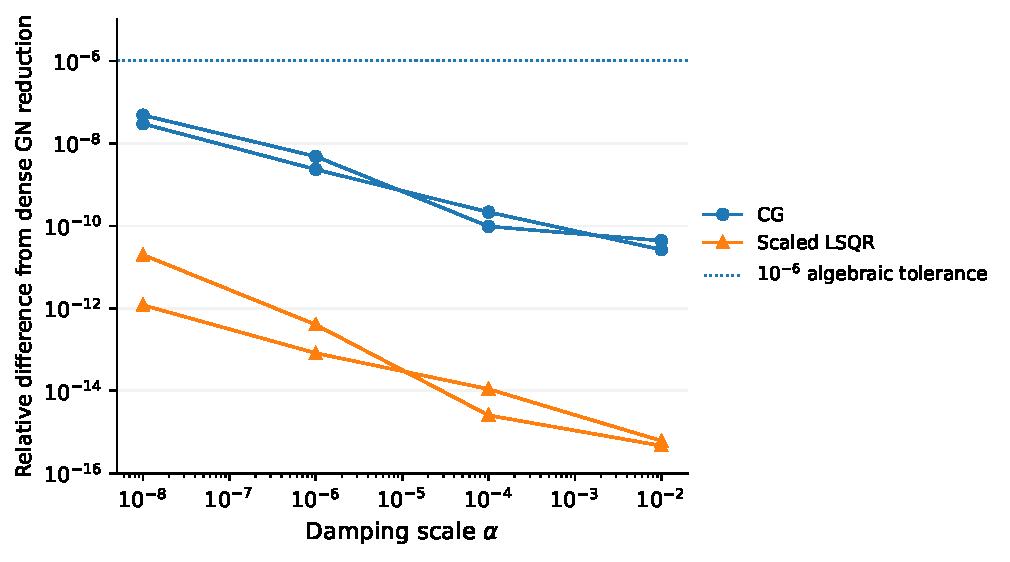
\includegraphics[width=.97\linewidth]{figures/fig05b_solver_agreement.pdf}
\caption{Relative discrepancy against dense Gauss--Newton reduction for CG and scaled augmented LSQR across both coupled checkpoints (seeds $215$ and $224$). Dense self-differences are zero and omitted on the logarithmic axis.}
\end{figure}

\section{Operator-scale matrix-free experiment}
To measure matrix-free scaling at large state dimensions without explicit Jacobian storage, a width-$25$ state network is expanded in a function-preserving manner (zero output weights on added hidden units) to hidden widths $250$, $2500$, and $25{,}000$, yielding $n_\theta\in\{1001, 10{,}001, 100{,}001\}$.
Residual grids are refined using real collocation, observation, initial, and boundary residuals ($m\in\{213, 853, 3413\}$, Table~S18).

\begin{table}[!htbp]
\centering\small
\caption{Residual grid constructions used in the operator-scale feasibility study.}
\begin{tabular}{rrrrr}
\toprule
$m$ & PDE grid & Data grid & Initial points & Boundary points per side\\\midrule
213 & $9\times9$ & $9\times9$ &17&17\\
853 & $19\times19$ & $19\times19$ &45&43\\
3413 & $39\times39$ & $39\times39$ &123&124\\\bottomrule
\end{tabular}
\end{table}
Matrix-free CG runs at $\alpha=10^{-2}$ with $20$ power iterations for $\lambda_{\max}(G_{\theta\theta})$, solve tolerance $10^{-10}$, verification gate $10^{-8}$, and a $500$-iteration cap.
All $27/27$ repeated solves pass verification.

\begin{figure}[!htbp]
\centering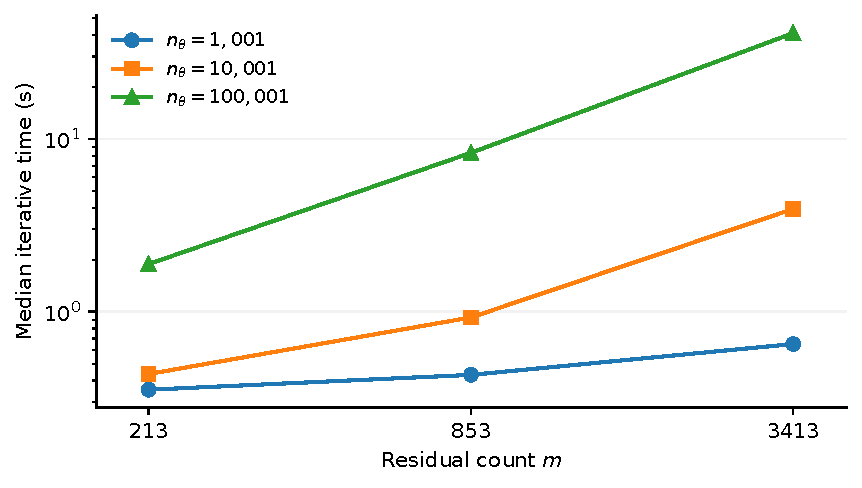
\includegraphics[width=.94\linewidth]{figures/s03_operator_scaling.pdf}
\caption{Median matrix-free CG iteration times across state dimensions $n_\theta\in\{1001,10{,}001,100{,}001\}$ and residual counts $m\in\{213,853,3413\}$ at $\alpha=10^{-2}$ (three repeats per grid cell on function-preserving expanded networks).}
\end{figure}
At the largest grid ($n_\theta=100{,}001$, $m=3413$), shared setup takes $62.83\text{ s}$ and median CG iteration time is $40.97\text{ s}$ ($103.80\text{ s}$ combined, excluding checkpoint loading, widening, and residual construction; CPU execution in \texttt{float64}, Python 3.12.13, PyTorch 2.13.0, NumPy 2.3.5).

\section{Equivalent energy audit and reproducibility checks}
For $M=J_\theta^\top J_\theta+\gamma I$, $Y=J_\lambda$, and an approximate state solve $\widehat Z=Z_\star+E$ with normal residual $R=M\widehat Z-J_\theta^\top Y=ME$, expanding the energy form $\widehat F_E=(Y-J_\theta\widehat Z)^\top(Y-J_\theta\widehat Z)+\gamma\widehat Z^\top\widehat Z$ cancels all linear cross terms via $MZ_\star=J_\theta^\top Y$, yielding
\begin{equation}
 \widehat F_E-F_{\rm se}^{\rm GN}=E^\top M E=R^\top M^{-1}R,\qquad
 0\preceq \widehat F_E-F_{\rm se}^{\rm GN}\preceq \gamma^{-1}R^\top R.
\end{equation}
This exact-arithmetic bound is a posteriori (computed from the returned residual $R$) and controls iterative solve error only; it does not enclose Gauss--Newton truncation, state-stationarity error, or floating-point roundoff, and can be conservative at very small $\gamma$.
Unit tests accompanying the codebase verify this algebraic identity, positive-semidefiniteness, the dominance inequality of Corollary~1, and exact consistency between exported CSV summaries and all manuscript tables and figures without requiring PINN retraining.
\end{document}
